% ====================================================================
% JAISP paper -- target: The Astrophysical Journal (ApJ)
% AASTeX v6.3.1.  Get the class from https://journals.aas.org/aastex-package-for-manuscripts/
% Build:  latexmk -pdf main.tex   (or pdflatex x3 + bibtex)
% ====================================================================
\documentclass[twocolumn]{aastex701}

\usepackage{amsmath,amssymb}
\usepackage{graphicx}
\graphicspath{{figures/}}

% --- convenience macros ---
\newcommand{\jaisp}{\textsc{Jaisp}}
\newcommand{\mas}{\,\mathrm{mas}}
\newcommand{\arcsecpx}{\arcsec\,\mathrm{px}^{-1}}
\newcommand{\todo}[1]{\textcolor{red}{[TODO: #1]}}
\usepackage{xcolor}

\shorttitle{A Joint Rubin--Euclid Foundation Model for Astrometry}
\shortauthors{Hemmati et al.}

\begin{document}

\title{Cross-Instrument Source Detection and Astrometry with a Joint Rubin--Euclid Foundation Model}

% ---- author block (placeholder) ----
\author{Shoubaneh Hemmati}
\affiliation{IPAC, California Institute of Technology, Pasadena, CA, USA}
\email{shemmati@ipac.caltech.edu}
% \author{...}\affiliation{...}
% \collaboration{...}

\begin{abstract}
% ABSTRACT -- draft
The Vera C.\ Rubin Observatory and \textit{Euclid} survey overlapping sky at
complementary wavelengths and resolutions, but their pixel-level data are
rarely combined before catalog construction. We present \jaisp{}, a joint
Rubin--\textit{Euclid} foundation model that ingests six Rubin optical bands
($ugrizy$) together with \textit{Euclid} VIS and NISP ($Y\!J\!H$) imagery at a
common fused resolution, and learns a shared representation by masked
reconstruction. We use the frozen representation to drive two downstream tasks
on $\sim$790 paired tiles in the ECDFS field: source detection with a
center-prediction head, and astrometry via a multi-band joint centroid that
fuses the sharp \textit{Euclid} VIS localization across all instruments.
% --- key results ---
The joint multi-band position reduces per-band centroid scatter relative to a
single-band measurement, with the largest gains at low signal-to-noise
($\sim$2.4--2.5$\times$ over a VIS-only anchor at $\mathrm{SNR}=5$ in a
controlled source-injection test), and is validated against \textit{Gaia} to
$4.4$--$4.8\mas$ at $G<18.5$. We critically examine what the foundation
contributes: through ablations and injection tests we find the cross-instrument
gain is genuine but bounded by the VIS localization floor, and that detection
completeness is suppressed near bright stars by the network's
signal-to-noise input normalization.
% --- OOD ---
Finally we report a first out-of-distribution test, applying the frozen model
without retraining to the EDF-S field: detection and \textit{Euclid} NISP
astrometry transfer cleanly, \todo{state final Rubin optical transfer result
after real-variance rerun}. \todo{one-sentence takeaway on the value of
multi-instrument pixel-level fusion.}

\end{abstract}

\keywords{Astrometry --- Surveys --- Convolutional neural networks --- Sky surveys
  --- Astronomy data analysis}

\section{Introduction}
\label{sec:intro}

% --- the opportunity ---
Rubin and \textit{Euclid} image overlapping sky with complementary strengths:
Rubin provides deep six-band optical photometry at ground-based resolution,
while \textit{Euclid} VIS delivers diffraction-limited optical morphology and
NISP adds near-infrared coverage. Jointly they constrain spectral energy
distributions and positions better than either alone, yet standard pipelines
process each instrument independently and combine only at the catalog level,
discarding pixel-level cross-instrument information.

% --- foundation models in astronomy: position relative to prior work ---
\todo{Position relative to prior astronomical foundation / multimodal
representation models (e.g.\ AstroCLIP, Multimodal Universe, AstroPT) and to
classical multi-instrument forced photometry / forced astrometry. Make the
novelty boundary explicit: pixel-level, multi-instrument, mixed-resolution
fusion driving downstream detection and astrometry.}

% --- what this paper does ---
In this paper we (i) describe \jaisp{}, a joint Rubin--\textit{Euclid}
foundation model trained by masked reconstruction on a common fused pixel grid
(\S\ref{sec:methods}); (ii) use the frozen representation for source detection
and for a multi-band joint-centroid astrometry that transfers the sharp
\textit{Euclid} VIS localization to bands where the source is faint
(\S\ref{sec:results}); (iii) validate positions against truth via
source injection and against \textit{Gaia}; and (iv) report a first
out-of-distribution evaluation on a second field with no retraining
(\S\ref{sec:ood}). Throughout we take a deliberately critical stance, using
ablations and controlled injections to separate what the multi-instrument
representation genuinely buys from what is already available in the single
sharpest band.

% --- contributions ---
Our main contributions are:
\begin{enumerate}
  \item A multi-instrument, mixed-resolution pixel-level foundation model for
    Rubin$+$\textit{Euclid}, with frozen-feature downstream heads.
  \item A multi-band joint-centroid astrometry method and a controlled
    quantification, via source injection, of the cross-instrument localization
    gain and its VIS-imposed ceiling.
  \item A first transfer (out-of-distribution) evaluation of the frozen stack
    on an independent field.
  \item Honest characterization of failure modes: foundation-version
    insensitivity, the VIS localization floor, and bright-star detection
    suppression.
\end{enumerate}

\section{Data}
\label{sec:data}

% --- fields ---
Our primary field is ECDFS (Rubin tract 5063), where we assemble
$\sim$790 paired Rubin$+$\textit{Euclid} tiles. \todo{exact tile count,
sky area, depth, epoch.} For the out-of-distribution test
(\S\ref{sec:ood}) we use 72 paired tiles in the EDF-S field
(tract 2394).

% --- bands and resolution ---
Each tile carries six Rubin bands ($ugrizy$) and four \textit{Euclid} bands
(VIS, NISP $Y$, $J$, $H$). \textit{Euclid} imagery is taken from the MER
mosaics; VIS and NISP are sampled at $0.1\arcsecpx$ ($\sim$1084$\times$1084
per tile), and Rubin at \todo{Rubin pixel scale / tile shape (6$\times$512$\times$512)}.
The native pixel scales and per-band World Coordinate Systems are retained;
the foundation model resamples internally to a common fused scale of
$0.4\arcsecpx$ (\S\ref{sec:methods}).

\begin{figure*}
  \centering
  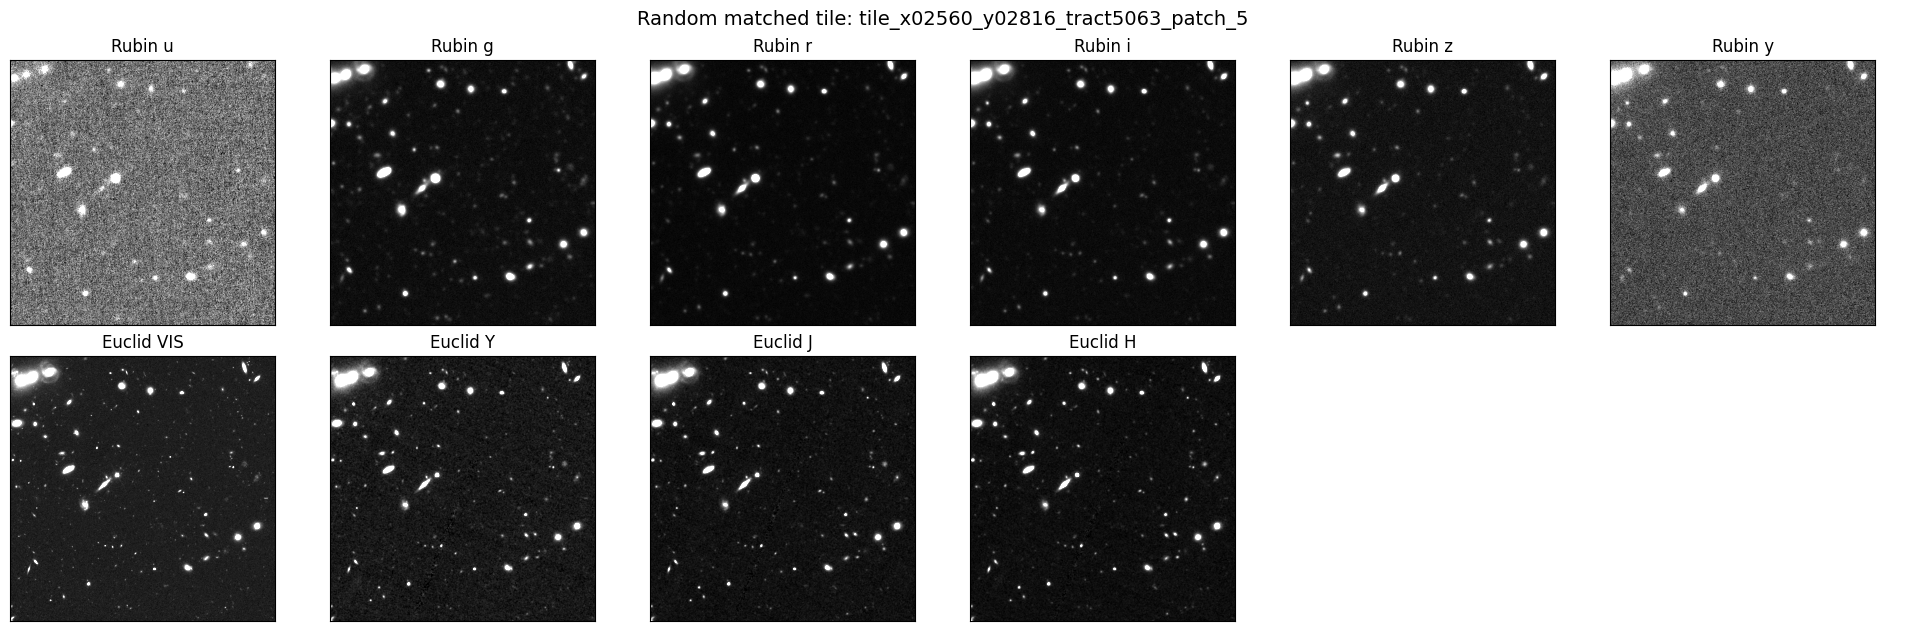
\includegraphics[width=\linewidth]{random_10bandtile.png}
  \caption{The ten input channels for a single matched tile. Top: Rubin
    $ugrizy$ ($512^2$ at $0.2\arcsecpx$). Bottom: \textit{Euclid} VIS and NISP
    $Y\!J\!H$ ($\sim$1084$^2$ at $0.1\arcsecpx$, from the MER mosaics). The
    sharp VIS channel and the depth and noise differences across bands are the
    raw material the foundation model fuses.}
  \label{fig:tile}
\end{figure*}

% --- variance / masks ---
Per-pixel variance maps accompany the Rubin imagery and, in the primary field,
the \textit{Euclid} imagery. \todo{Note: the EDF-S \textit{Euclid} tiles used
for the first OOD pass lacked variance maps; see \S\ref{sec:ood}. State final
data state after real-variance tiles are obtained.}

% --- truth / external catalogs ---
For astrometric validation we use \textit{Gaia} \todo{DR} as an absolute
reference, and \todo{the \textit{Euclid} MER catalog for detection
completeness/purity}. We additionally construct a controlled
source-injection set (\S\ref{sec:results}) to measure positional error against
known truth.

\section{Methods}
\label{sec:methods}

\subsection{The \jaisp{} foundation model}
\label{sec:methods:foundation}

% --- architecture ---
\jaisp{} encodes each band with a per-band convolutional stem, resamples the
per-instrument streams to a common fused pixel scale of $0.4\arcsecpx$, and
fuses them into a shared bottleneck representation. \todo{Architecture detail:
per-band stems, mixed-resolution stream depths from $\log_2$(scale ratio),
ConvNeXt/transformer blocks, FiLM band conditioning, concat fusion (v9/v10).}
The per-band stem normalizes its input by the per-pixel noise,
$x = \mathrm{image}/\mathrm{rms}$, and clamps the result to a fixed
signal-to-noise range before feature extraction; this choice is revisited in
\S\ref{sec:results} as the origin of bright-star detection suppression.

% --- training ---
The model is trained by masked reconstruction \todo{(MAE objective, masking
fraction, cross-instrument masking, Charbonnier$+$core-L2 loss for v10), epochs,
optimizer, hardware}. All downstream heads operate on \emph{frozen} features.

% --- versions / equivalence note ---
\todo{Briefly: several architecture variants (v8 fine-scale, v9 concat fusion,
v10 loss-shaped) were trained; in-distribution probes and downstream metrics
find them statistically equivalent (see \S\ref{sec:discussion}). Report the
production checkpoint used here (v10 warm-start).}

\subsection{Detection head}
\label{sec:methods:detection}

% --- centernet ---
We detect sources with a center-prediction (CenterNet-style) head on the frozen
fused features, producing a normalized centroid and score per source.
\todo{Head architecture, self-training/pseudo-label procedure, operating point
(conf threshold), NMS.} Detections are gated on the \textit{Euclid} VIS signal
and serve as seeds for astrometry.

\subsection{Multi-band joint-centroid astrometry}
\label{sec:methods:astrometry}

% --- the instrument ---
Given a detection seed, we (i) refine the centroid classically on
\textit{Euclid} VIS, (ii) solve for a single \emph{joint canonical} sky
position by simultaneously fitting the source across all bands, weighting each
band by its noise and accounting for its PSF, and (iii) measure each band's
classical centroid and record its offset from the joint canonical position.
The joint canonical position is the cross-instrument estimate; the per-band
offset is the astrometric residual we report.

% --- why this beats single-band ---
Because the fit is dominated by the band with the sharpest, highest-SNR
localization (typically \textit{Euclid} VIS), the joint position transfers that
localization to bands in which the source is faint or unresolved
(\S\ref{sec:results}). Per-source uncertainties follow from the $\chi^2$
curvature of the joint fit and a per-band $\mathrm{FWHM}/(2.355\,\mathrm{SNR})$
centroid-noise model.

% --- foundation-agnostic note ---
We emphasize that step (i)--(iii) are classical given the detection seeds; the
foundation's role in astrometry is to supply the cross-instrument detections.
A learned per-object position head was also trained and is discussed as an
ablation in \S\ref{sec:discussion}.

\section{Results on ECDFS}
\label{sec:results}

\subsection{Detection}
\label{sec:results:detection}

% --- detection numbers ---
On the $\sim$790 ECDFS tiles the detector returns $\sim$413 sources per tile at
the chosen operating point (Fig.~\ref{fig:detection}). \todo{Completeness/purity
against a reference catalog; comparison to a classical VIS baseline
(notebook 06).}

\begin{figure}
  \centering
  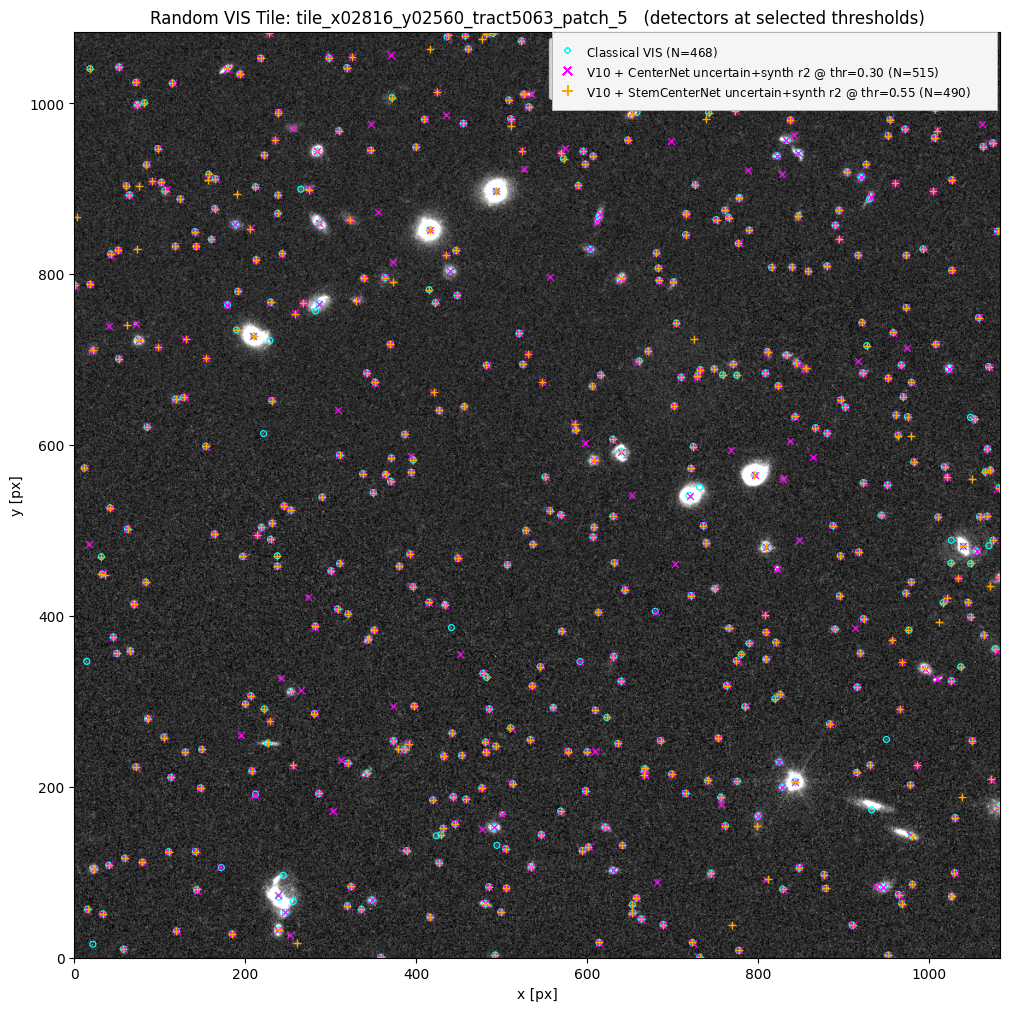
\includegraphics[width=\linewidth]{detection_v10_selected_threshold_overlay.png}
  \caption{Detections on a representative \textit{Euclid} VIS tile at the
    selected operating point: the classical VIS reference, the fused
    center-prediction head, and the native-resolution stem head. \todo{Tighten
    legend / crop; add a zoom-in panel near a bright star to motivate
    \S\ref{sec:results:detection}.}}
  \label{fig:detection}
\end{figure}

% --- bright star suppression ---
Detection completeness is reduced near bright stars: the source count per tile
anticorrelates with the fraction of the tile under bright extended flux
($\mathrm{corr}=-0.46$). We trace this to the per-band stem normalization
(\S\ref{sec:methods:foundation}): a saturated star produces a wide region
pinned at the clamped signal-to-noise ceiling, which dominates the group-wise
feature normalization and depresses faint-source activations. We verify this is
\emph{not} a removable smooth background (subtracting a spatially varying
background changes the count negligibly) and that it is intrinsic to the
detector rather than a noise-model artifact. \todo{Quantify against MER truth:
are the lost sources real?}

\subsection{Astrometry: per-band residual and SNR scaling}
\label{sec:results:astro}

% --- headline numbers ---
The joint-centroid astrometry reduces the pooled per-band median residual from
$\sim$50$\mas$ (raw band-vs-canonical, dominated by per-band centroid scatter)
to $\sim$11--16$\mas$ per band ($\sim$11$\mas$ pooled in the NISP and red
optical bands; Fig.~\ref{fig:astro_perband}). The residuals follow the expected
$\mathrm{FWHM}/(2.355\,\mathrm{SNR})$ centroid-noise scaling
(Fig.~\ref{fig:snr}), reaching \todo{floor at high SNR}.

\begin{figure}
  \centering
  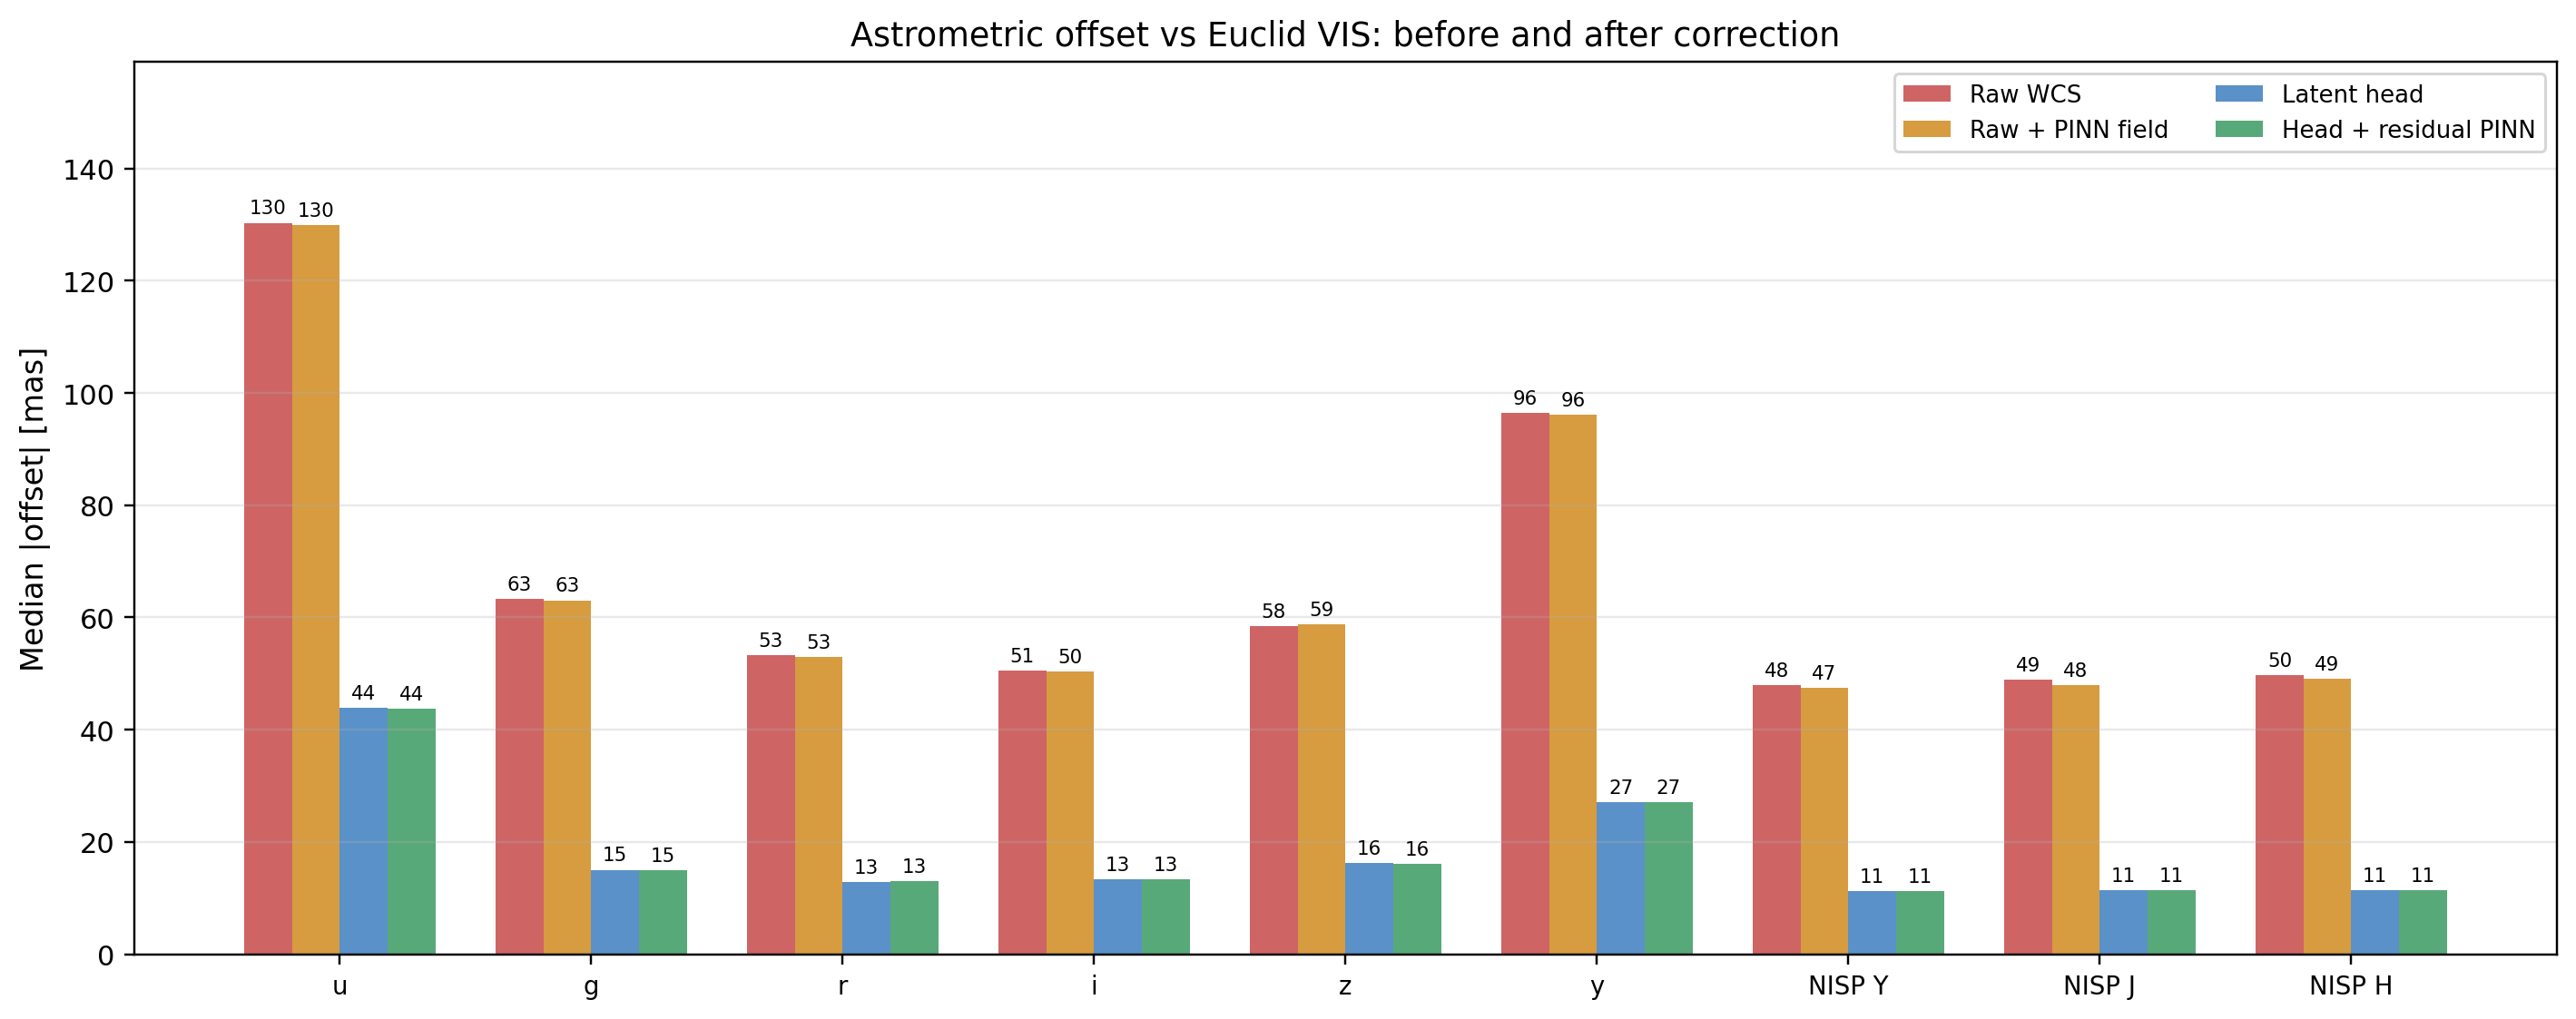
\includegraphics[width=\linewidth]{astrometry_before_after.png}
  \caption{Median per-band astrometric offset to the \textit{Euclid} VIS
    reference, before and after correction. The raw cross-instrument offset
    (red) ranges from $\sim$50$\mas$ in the red optical bands to $130\mas$ in
    $u$; the per-object correction (blue) brings every band to
    $\sim$11--16$\mas$, with NISP reaching $11\mas$. The smooth concordance
    field alone (orange) removes little of the per-source scatter, confirming
    the residual is dominated by object-level centering, not a bulk WCS term.
    \todo{Confirm whether the per-band panel should show the joint-centroid
    instrument rather than the latent-head ablation shown here (see text).}}
  \label{fig:astro_perband}
\end{figure}

\subsection{Source-injection truth test}
\label{sec:results:injection}

% --- injection ---
To measure positional error against known truth we inject sub-pixel point
sources across all ten bands at a range of signal-to-noise levels and recover
their positions with the same pipeline. At $\mathrm{SNR}=5$ (Rubin) the
classical single-band centroid errs by $\sim$47$\mas$, the joint/canonical
position by $\sim$18--19$\mas$, approaching the VIS-only localization floor of
$\sim$17$\mas$; a position fitted jointly across all bands improves on a
VIS-only anchor by $\sim$2.4--2.5$\times$ ($16.6\rightarrow6.7\mas$ at peak
$\mathrm{SNR}=5$). \todo{Confirm numbers, add table, state caveats: idealized
Gaussian PSFs, isolated sources, injected NISP sharper than the real MER PSF.}
The test also bounds the gain: where a band is intrinsically sharper than VIS,
transferring the VIS position degrades rather than improves it
(\S\ref{sec:discussion}).

\begin{figure}
  \centering
  
\includegraphics[width=\linewidth]{astrometry_truth_vs_snr.png}
  \caption{Astrometric error versus true position from controlled
    source injection into held-out tiles (Rubin bands). The classical
    single-band centroid (red) is the no-fusion baseline; the joint multi-band
    position approaches the \textit{Euclid} VIS-only localization floor (brown
    dashed), and the joint ten-band classical fit (green) is the production
    position instrument. The latent-head curves (blue/purple) overlap at the
    faint end, showing the head's $\sim$17--18$\mas$ floor is intrinsic, not
    label-limited. The dotted line marks the $\sim$4--7$\mas$ scale of the real
    concordance field (\S\ref{sec:results:field}).}
  \label{fig:snr}
\end{figure}

\subsection{Absolute validation against \textit{Gaia}}
\label{sec:results:gaia}

% --- gaia ---
Cross-matching the joint canonical positions to \textit{Gaia} gives a bulk
offset of $(+3.7, +1.9)\mas$ and a per-star scatter of $\sim$5.4$\mas$ after
bulk removal, improving to $4.4$--$4.8\mas$ for $G<18.5$. \todo{Gaia DR,
matching radius, N, magnitude-binned table, spatial structure of the offset.}

\subsection{A coherent cross-survey concordance field}
\label{sec:results:field}

% --- the field ---
After removing the bulk offset, the per-band residuals between the Rubin and
\textit{Euclid} astrometric solutions are not spatially random: they trace a
smooth, coherent field across the survey footprint. Decomposing the matched
source offsets with a multi-scale field solver, we isolate a degree-scale
component of amplitude $\sim$4--7$\mas$ that varies slowly across the field
(Fig.~\ref{fig:field}). This is the residual mismatch between the two
instruments' independently solved World Coordinate Systems --- precisely the
unmodeled structure that classical per-instrument pipelines, which calibrate
each survey's astrometry separately, leave in place
(\S\ref{sec:intro}, SITCOMTN-159).

% --- why we trust it ---
We establish that this degree-scale field is a real measurement and not solver
noise: it is recovered consistently across independent fits, across the choice
of duplicate handling, across reference catalogs, and --- importantly --- across
\jaisp{} foundation-model versions, with the smoothed field agreeing at Pearson
$r$ up to $0.92$. \todo{State the smoothing scale ($\sim$150\arcsec) and the
cross-comparison numbers; reference the controlled refit audit.}

% --- honest bound ---
We are deliberate about what is and is not established. Only the degree-scale
component is reproducible; sub-degree structure in any single solver product
sits below the solver's run-to-run repeatability floor ($\sim$5$\mas$) and is
not interpretable. We therefore report the field as a characterized
\emph{measurement} of the cross-survey WCS residual, not as a production
correction applied to the catalog.

\begin{figure}
  \centering
  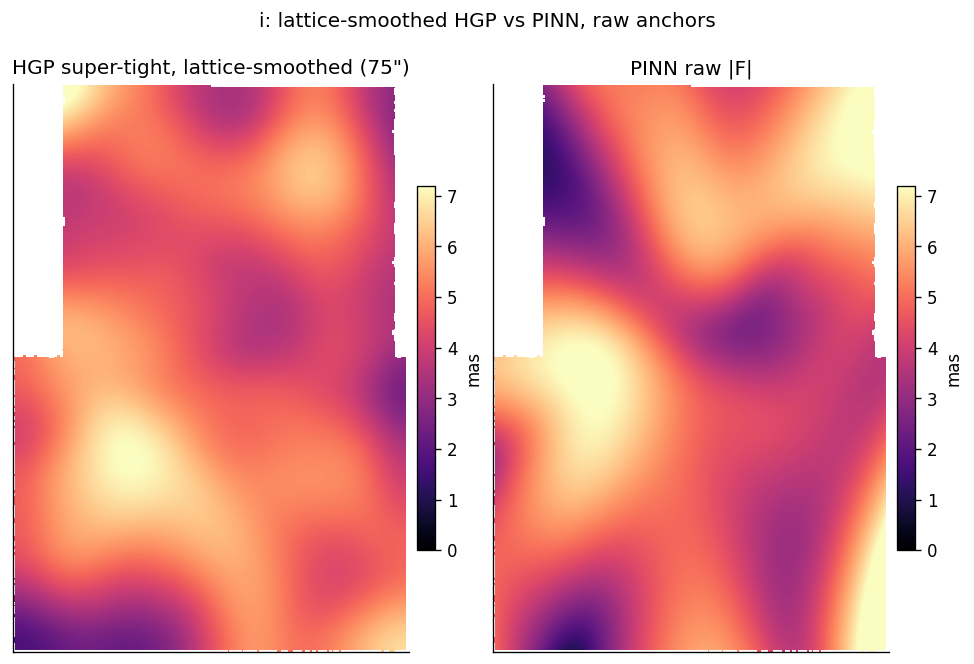
\includegraphics[width=\linewidth]{hgp_lattice_smoothed_vs_pinn.png}
  \caption{The degree-scale cross-survey concordance field (\textit{i} band),
    recovered two independent ways from the matched per-band residuals: a
    lattice-smoothed hierarchical-GP fit (left) and a physics-informed
    smooth-field fit (right). Both recover the same $\sim$4--7$\mas$ large-scale
    topology; their agreement at this scale --- and across foundation-model
    versions --- is the evidence that the field is a property of the data rather
    than solver noise. \todo{Optionally add the cross-version overlay /
    correlation panel.}}
  \label{fig:field}
\end{figure}

\section{Out-of-Distribution Transfer: EDF-S}
\label{sec:ood}

% --- motivation ---
The value proposition of a foundation model is transfer without retraining. All
results above are in the ECDFS field on which the downstream heads were tuned.
Here we apply the frozen \jaisp{} stack --- foundation, detector, and
joint-centroid astrometry --- to 72 paired tiles in the independent EDF-S field
(tract 2394) with no retraining or refitting.

% --- caveat on this pass ---
\todo{State the final data condition. The first pass used \textit{Euclid} tiles
without variance maps, requiring a median-absolute-deviation RMS fallback for
VIS/NISP (Rubin variance was present and used directly). Results below are
either (a) to be reported on real-variance tiles, or (b) reported with the
fallback and the real-variance rerun as a robustness check.}

% --- what transfers ---
Detection transfers cleanly (456 sources per tile versus 413 on ECDFS; no
processing errors), and \textit{Euclid} NISP astrometry matches the
in-distribution residual ($35$--$41\mas$ versus $40\mas$). The signal-to-noise
scaling of the residual is reproduced. \todo{Final Rubin optical
($g\,r\,i\,z$) transfer result: the first (fallback) pass showed a
$\sim$1.5$\times$ larger matched-SNR residual whose origin --- the RMS fallback
perturbing the joint-fit weighting versus genuine field differences --- is
resolved by the real-variance rerun. Report the resolved outcome here.}

\begin{figure}
  \centering
  % \includegraphics[width=\linewidth]{ood_astrometry_compare.png}
  \caption{Per-band and SNR-binned astrometric residual, EDF-S (OOD) versus
    ECDFS. \todo{final figure from notebook 15.}}
  \label{fig:ood}
\end{figure}

% --- detection completeness OOD ---
The bright-star detection suppression (\S\ref{sec:results:detection})
reproduces and is somewhat stronger in EDF-S ($\mathrm{corr}=-0.71$),
consistent with its origin in the input normalization rather than the field.
\todo{MER-catalog completeness in EDF-S.}

\section{Discussion}
\label{sec:discussion}

\subsection{What the multi-instrument representation actually buys}
% --- the honest core ---
The cross-instrument gain is real but bounded. The joint position improves
faint-band localization because it imports the sharpest available
(\textit{Euclid} VIS) constraint; it adds no precision beyond that band, and
where another band is intrinsically sharper, transferring the VIS position is
counterproductive (\S\ref{sec:results:injection}). The practical value is
therefore largest exactly where it is most needed: measuring positions in bands
where a source is too faint to localize on its own.

\subsection{Foundation-version insensitivity}
% --- negative result, stated plainly ---
We trained several foundation variants (\S\ref{sec:methods:foundation}).
In-distribution linear probes and downstream detection/astrometry metrics do
not statistically distinguish them. \todo{Quantify.} We argue the
discriminating test for foundation quality is out-of-distribution transfer
(\S\ref{sec:ood}) rather than in-distribution downstream accuracy, which
saturates against label noise.

\subsection{Label noise and the limits of in-distribution metrics}
\todo{Summarize the centroid-emulation finding: at the faint end the
band-vs-canonical residual measures the model reproducing the canonical
centroid definition, not positional truth; this is why injection and
\textit{Gaia} (truth metrics) are necessary and in-distribution residuals are
not sufficient.}

\subsection{Bright-star detection suppression}
% --- mechanism + fix ---
The signal-to-noise input normalization that stabilizes training also lets a
saturated star dominate the local feature statistics, suppressing faint
detections nearby (\S\ref{sec:results:detection}). This is a completeness, not
an astrometric-accuracy, effect. Mitigations --- local background subtraction,
a bright-star-aware rescue pass, or a normalization less sensitive to saturated
outliers --- are left to future work. \todo{If MER shows the lost sources are
real, quantify the completeness cost and any mitigation tested.}

\subsection{Limitations}
\begin{itemize}
  \item Injection uses idealized PSFs and isolated sources; blends and
    realistic wings are not captured.
  \item Out-of-distribution evidence is from a single second field.
  \item \todo{variance-map availability; Rubin optical transfer; others.}
\end{itemize}

\section{Summary}
\label{sec:summary}

We presented \jaisp{}, a joint Rubin--\textit{Euclid} foundation model operating
on a common fused pixel grid, and used its frozen representation for source
detection and multi-band joint-centroid astrometry. Our main findings:

\begin{enumerate}
  \item A joint multi-band position transfers the sharp \textit{Euclid} VIS
    localization to faint bands, improving low-SNR positions by
    $\sim$2.4--2.5$\times$ over a single-band measurement in controlled
    injection tests, and validating against \textit{Gaia} to $4.4$--$4.8\mas$
    at $G<18.5$.
  \item The gain is bounded by the VIS localization floor; the representation
    adds no precision beyond the sharpest contributing band.
  \item The frozen stack transfers to an independent field without retraining
    for detection and \textit{Euclid} NISP astrometry; \todo{final Rubin
    optical transfer statement.}
  \item Detection completeness is suppressed near bright stars by the input
    normalization, a characterized and mitigable effect.
\end{enumerate}

\todo{Closing sentence on the role of pixel-level multi-instrument fusion for
Rubin$+$\textit{Euclid} survey science, and next steps (additional fields,
photometry, weak-lensing shapes).}


\begin{acknowledgments}
\todo{acknowledgments, facilities, software}
\end{acknowledgments}

\facilities{Rubin Observatory, Euclid}
\software{Astropy \citep{astropy2022}, NumPy, SciPy, PyTorch, SEP \citep{barbary2016}}

\bibliographystyle{aasjournalv7}
\bibliography{refs}

\end{document}
